\documentclass[xcolor=dvipsnames
              ,handout
              ]{beamer} 

\usetheme{Madrid} 
%\setbeamertemplate{blocks}[shadow=false] 
\setbeamertemplate{navigation symbols}{} 
\setbeamertemplate{items}[square]
\setbeamertemplate{sections/subsections in toc}[square]

\definecolor{myblueend}{rgb}{0.058,0.132,0.42}
\definecolor{mybluemiddle}{rgb}{0.31,0.45,0.64}
\definecolor{mybluestart}{rgb}{0.17,0.28,0.48}
\definecolor{mygreen}{rgb}{0,0.7,0}
\definecolor{mylightgreen}{rgb}{0.7,1,0.7}
\definecolor{mylightblue}{rgb}{0.7,0.7,1}
\definecolor{mylightblack}{rgb}{0.7,0.7,0.7}
\definecolor{mylightred}{rgb}{1,0.7,0.7}
\definecolor{oproverblue}{RGB}{12,83,144}
\definecolor{oproveryellow}{RGB}{255,156,55}
\definecolor{mydarkgreen}{rgb}{0.17,0.48,0.28}
\definecolor{mydarkred}{rgb}{0.48,0.28,0.17}
\definecolor{grey}{rgb}{0.7,0.7,0.7}

%\setbeamercolor{palette primary}{fg=white,bg=mybluestart}
%\setbeamercolor{palette secondary}{fg=white,bg=mybluestart}
%\setbeamercolor{palette tertiary}{fg=white,bg=mybluestart}
%\setbeamercolor{palette quaternary}{fg=white,bg=mybluestart}
\setbeamercolor{palette primary}{fg=white,bg=oproverblue}
\setbeamercolor{palette secondary}{fg=white,bg=oproverblue}
\setbeamercolor{palette tertiary}{fg=white,bg=oproverblue}
\setbeamercolor{palette quaternary}{fg=white,bg=oproverblue}
\setbeamercolor{titlelike}{parent=palette quaternary}

\setbeamercolor{item}{fg=oproverblue}
\setbeamercolor{block title}{fg=white,bg=oproverblue}
\setbeamercolor{block title example}{fg=white,bg=oproveryellow}
%\setbeamercolor{block title alert}{fg=white,bg=mydarkred}

\usefonttheme{serif}

%%
%% TOOLS
%% 
\newcommand{\opensmt}{{\sc OpenSMT}\xspace}
\newcommand{\yices}{{\sc Yices}\xspace}
\newcommand{\mathsat}{{\sc MathSAT}\xspace}
\newcommand{\cvcfour}{{\sc CVC4}\xspace}
\newcommand{\zthree}{{\sc Z3}\xspace}
\newcommand{\boolector}{{\sc Boolector}\xspace}
\newcommand{\verit}{{\sc veriT}\xspace}
\newcommand{\stp}{{\sc STP}\xspace}
\newcommand{\minisat}{{\sc MiniSAT}\xspace}
%%
%% BOOLEAN OPERATORS
%%
\newcommand{\swedge}{\,\wedge\,}
\newcommand{\svee}{\,\vee\,}
\newcommand{\impl}{\,\rightarrow\,}
%%
%% SMTLIB LOGICS
%% 
\newcommand{\Idl}{\ensuremath{\mathcal{IDL}}\xspace}
\newcommand{\Rdl}{\ensuremath{\mathcal{RDL}}\xspace}
\newcommand{\Uf}{\ensuremath{\mathcal{UF}}\xspace}
\newcommand{\Lia}{\ensuremath{\mathcal{LIA}}\xspace}
\newcommand{\Lra}{\ensuremath{\mathcal{LRA}}\xspace}
\newcommand{\Arrays}{\ensuremath{\mathcal{A}}\xspace}
\newcommand{\Bitvectors}{\ensuremath{\mathcal{BV}}\xspace}
\newcommand{\T}{\ensuremath{\mathcal{T}}\xspace}
\newcommand{\B}{\ensuremath{\mathcal{B}}\xspace}
%%
%% SETS
%%
\newcommand{\Int}{\ensuremath{\mathbb{Z}}\xspace}
\newcommand{\Rat}{\ensuremath{\mathbb{Q}}\xspace}
\newcommand{\Rea}{\ensuremath{\mathbb{R}}\xspace}
\newcommand{\Boo}{\ensuremath{\mathbb{B}}\xspace}
%%
%% SORTS
%%
\newcommand{\SInt}{{\tt Int}\xspace}
\newcommand{\SRea}{{\tt Real}\xspace}
\newcommand{\SBoo}{{\tt Bool}\xspace}
\newcommand{\SBv}[1]{{\tt BV}$_{[#1]}$\xspace}
%%
%% SMT specific
%%
\newcommand{\tconflict}{\T-conflict\xspace}
\newcommand{\tconflicts}{\T-conflicts\xspace}
\newcommand{\tterm}{\T-term\xspace}
\newcommand{\tterms}{\T-terms\xspace}
\newcommand{\tatom}{\T-atom\xspace}
\newcommand{\tatoms}{\T-atoms\xspace}
\newcommand{\tlit}{\T-literal\xspace}
\newcommand{\tlits}{\T-literals\xspace}
\newcommand{\tformula}{\T-formula\xspace}
\newcommand{\batom}{\B-atom\xspace}
\newcommand{\batoms}{\B-atoms\xspace}
\newcommand{\blit}{\B-literal\xspace}
\newcommand{\blits}{\B-literals\xspace}
\newcommand{\babst}[1]{#1^{\B}}
\newcommand{\tsolver}{\T-solver\xspace}
\newcommand{\tsolvers}{\T-solvers\xspace}
%%
%% SAT specific
%%
\newcommand{\dec}[2]{\stackrel{\textcolor{oproveryellow}{#2}}{#1}}
%%
%% BIT-VECTORS
%%
\newcommand{\w}[2]{\ensuremath{#1_{[#2]}}}
\newcommand{\band}{\,{\bf AND}\,}
\newcommand{\bor}{\,{\bf OR}\,}
\newcommand{\bnot}{{\bf NOT}\,}
\newcommand{\bitandsymb}{\,\, {\bf AND}}
\newcommand{\bit}[2]{#1\ensuremath{^#2}}
%%
%% IDL graphs
%%
\newcommand{\idlnode}[2]{\frac{#1}{#2}}
%%
%% LRA Solver
%%
\newcommand{\bas}{\ensuremath{\mathcal{B}}\xspace}
\newcommand{\nonbas}{\ensuremath{\mathcal{N}}\xspace}
%%
%% EUF graphs
%%
%\newcommand{\nod}[3]{\frac{{#1}}{#2,#3}}
\newcommand{\nod}[3]{
  \tiny
  \begin{array}{c}
    #1 \\
    #2, #3
  \end{array}
}
%%
%% MISC
%%
\newcommand{\Lbrack}{\ensuremath{[\mspace{-3mu}[}}
\newcommand{\Rbrack}{\ensuremath{]\mspace{-3mu}]}}
\newcommand{\inter}[1]{\ensuremath{\Lbrack #1 \Rbrack}}
\newcommand{\COMMENT}[1]{}
\newcommand{\hl}[1]{\colorbox{oproveryellow}{\bf #1}}
\newcommand{\colfou}[1]{\textcolor{grey}{#1}}
\newcommand{\formulae}{formul\ae\xspace}
\newcommand{\smtsolvers}{SMT-solvers\xspace}
\newcommand{\smtsolver}{SMT-solver\xspace}
\newcommand{\satsolvers}{SAT-solvers\xspace}
\newcommand{\satsolver}{SAT-solver\xspace}
\newcommand{\bitvectors}{Bit-Vectors\xspace}
\newcommand{\bitvector}{Bit-Vector\xspace}
\newcommand{\colone}[1]{\textcolor{red}{#1}}
\newcommand{\coltwo}[1]{\textcolor{mygreen}{#1}}
\newcommand{\coloneat}[2]{\textcolor<#2>{red}{#1}}
\newcommand{\coltwoat}[2]{\textcolor<#2>{mygreen}{#1}}
\newcommand{\colfouat}[2]{\textcolor<#2>{grey}{#1}}
\newcommand{\claset}{\mathcal{C}}
\newcommand{\ra}[1]{\renewcommand{\arraystretch}{#1}}

\usepackage{epsfig}
\usepackage{graphicx}
\usepackage{color}
\usepackage{amstext}
\usepackage{amssymb}
\usepackage{amsfonts}
\usepackage{amsmath}
\usepackage{amsthm}
\usepackage{xspace}
\usepackage{multirow}
\usepackage{tabularx,colortbl}
\usepackage{alltt}
\usepackage{bussproofs}
\usepackage{algorithm2e}
\usepackage{datetime}


\title[\tsolver for \Uf]{Satisfiability Modulo Theories\\ Lecture 7 - A Theory Solver for \Uf \\ {\tiny (slides revision: \today, \currenttime)}}
\author[R. Bruttomesso]{\large Roberto Bruttomesso}
\date{1 Dicembre 2011}
\institute[SMT]{\large Seminario di Logica Matematica \\ (Corso Prof. Silvio Ghilardi)}
\logo{ \vspace{-6pt} 
\includegraphics[scale=0.15]{imgs/logo-ita.png} }

\begin{document}

\frame{\titlepage}

\begin{frame}
  \frametitle{Outline}
  \tableofcontents
\end{frame}

\section{Basics}
\subsection{Introduction}
\begin{frame}
  \frametitle{Introduction}

  Model-Checking is a set of techniques to approach the verification
  of a system (e.g., a hardware circuit, a program, a protocol)
  \vfill
  It was proposed by Clarke-Emerson and Sifakis-Quine
  as a way of automatically prove properties of a system
  \vfill
  The authors received the Turing Award in 2007
  \vfill
  The idea of model-checking was in 
  contrast with the established ``philosophy'' at that time ($\sim$ 1980) 
  which was suggesting semi-automatic human-driven approaches: 
  MC is loved by industry because of this ``push-button'' characteristic

\end{frame}

\subsection{Union-Find}
\begin{frame}
  \frametitle{Handling equalities: Union Find}

  \vfill
  Let's focus first on conjunctions of positive equalities 
  between variables, (functions, congruence, and negated
  equalities are not considered for the moment)
  \vfill\pause
  Union-Find algorithms (Tarjan). It is based on the notion
  of {\bf equivalence classes}. Equivalence classes
  form a partition of the set of variables $V$, i.e.,
  \begin{itemize}
    \item each partition is non empty
    \item each partition is disjoint
    \item the union of the partitions is $V$
  \end{itemize}
  \vfill\pause
  Let $\varphi^+$ be a conjunction of positive equalities: 
  Union-Find will find the partition of $V$ such that:
  \vfill
  \begin{center}
    $x$, $y$ are in the same partition iff $\varphi^+ \Rightarrow x=y$
  \end{center}

\end{frame}

\begin{frame}
  \frametitle{Union-Find}

  Input: a conjunction of positive equalities $\varphi^+$\\
  (e.g., $\varphi^+ \equiv\ x\!=\!y\ \wedge\ w\!=\!a\ \wedge\ w\!=\!b$, $V \equiv \{ x,y,w,z,a,b,c \}$) 
  \vfill
  Initialization: one equivalence class per each variable in $V$
  $$
  \{\ {\bf x}\ \}\quad\quad\{\ {\bf y}\ \}\quad\quad\{\ {\bf z}\ \}\quad\quad
  \{\ {\bf w}\ \}\quad\quad\{\ {\bf a}\ \}\quad\quad\{\ {\bf b}\ \}\quad\quad\{\ {\bf c}\ \}
  $$
  \vfill\pause
  For each equality $s=t$ in $\varphi^+$, merge the class containing $s$ with that containing $t$ (e.g., $x=y$)
  $$
  \{\ {\bf x}, y\ \}\quad\quad\{\ {\bf z}\ \}\quad\quad\{\ {\bf w}\ \}\quad\quad\{\ {\bf a}\ \}\quad\quad\{\ {\bf b}\ \}\quad\quad\{\ {\bf c}\ \}
  $$
  \vfill\pause
  The final situation is the desired partition
  $$
  \{\ {\bf x}, y\ \}\quad\quad\{\ {\bf z}\ \}\quad\quad\{\ w, {\bf a}, b\ \}\quad\quad\{\ {\bf c}\ \}
  $$
  Notice that $\varphi^+ \Rightarrow s=t$ iff $s$, $t$ in the same partition
  \vfill
  A variable per class is nominated {\bf representant}

\end{frame}

\begin{frame}[fragile]
  \frametitle{Implementing Union-Find}

  \scriptsize

  We assume each variable $x$ is a {\tt Node * x}
  \begin{columns}
  \begin{column}{.7\textwidth}
  \begin{verbatim}
    struct Node { 
      int    size;     // Keep track of a class size
      int    rank;     // Keep track of a class rank
      Node * root;     // Points to class' representant
    };
  \end{verbatim} 
  \end{column}
  \begin{column}{.3\textwidth}
    \begin{center}
    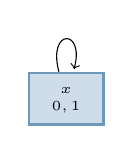
\begin{tikzpicture}[auto]

%
% Styles
%
\tikzstyle{vertex} = [rectangle,draw=oproverblue!60,fill=oproverblue!20,thick]

\node[vertex] (x) at ( 0, 0)  {$\nod{x}{0}{1}$};

\path (x) edge [loop above] (x);

\end{tikzpicture}

    \end{center}
  \end{column}
  \end{columns}
  initialized with size = 1, rank = 0, and root = $x$ 
  \vfill
  \begin{columns}

  \begin{column}{.45\textwidth}
    \pause
    \begin{overlayarea}{.44\textwidth}{4cm}
    \only<2-4|handout:0>{
    \begin{tabbing}
      asd \= ad \= sd \= asd \kill
      1 \> {\bf procedure} Union( $x$, $y$ ) \\
      2 \> assert( $x$ == $x$.root \&\& $y$ == $y.root$ ) \\
      3 \> if ( $x$ == $y$ ) return \\
      4 \> $x$.root = $y$ \\
      \\
      \\
      \\
      \\
      \\
      \\
      \\
      \\
      \\
    \end{tabbing}
   }
    \only<5>{
    \begin{tabbing}
      asd \= ad \= sd \= asd \kill
      1 \> {\bf procedure} Union( $x$, $y$ ) \\
      2 \> assert( $x$ == $x$.root \&\& $y$ == $y.root$ ) \\
      3 \> if ( $x$ == $y$ ) return \\
      4 \> if ( $x$.rank $<$ $y$.rank ) \\
      5 \> \> $x$.root = $y$ \\
      6 \> \> $y$.size = $y$.size $+$ $x$.size \\
      7 \> else if ( $x$.rank $>$ $y$.rank ) \\
      8 \> \> $y$.root = $x$ \\
      9 \> \> $x$.size = $x$.size $+$ $y$.size \\
     10 \> else \\
     11 \> \> $x$.root = $y$ \\
     12 \> \> $x$.size = $x$.size $+$ $y$.size \\
     13 \> \> $x$.rank = $x$.rank $+ 1$ \\
    \end{tabbing}
   }
   \end{overlayarea}
  \end{column}
  
  \begin{column}{.35\textwidth}
    \pause
    \begin{tabbing}
      asd \= ad \= sd \= asd \kill
      1 \> {\bf procedure} Find( $x$ ) \\
      2 \> $r = x$ \\
      3 \> if ( $r$ $\not=$ $r$.root ) \\
      4 \> \> $r$ = Find( $r$.root ) \\
      5 \> return $r$ \\
      \\
      \pause\\
      1 \> {\bf procedure} Union-Find( $\varphi^+$ ) \\
      2 \> foreach ( $x=y \in \varphi^+$ ) \\  
      3 \> \> $x =$ Find( $x$ ) \\
      4 \> \> $y =$ Find( $y$ ) \\
      5 \> \> Union( $x$, $y$ )
    \end{tabbing}
  \end{column}

  \end{columns}

\end{frame}

\begin{frame}
  \frametitle{Example}

  \scriptsize

  $\varphi^+ \equiv\ x\!=\!y\ \wedge\ w\!=\!a\ \wedge\ w\!=\!b$
  \vfill
  \begin{center}
  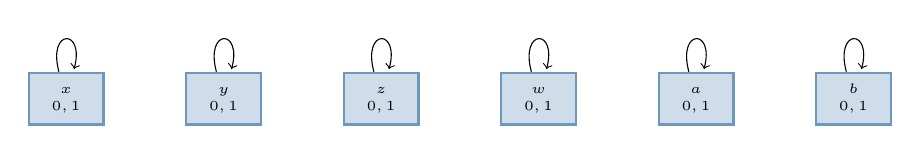
\begin{tikzpicture}[auto]

%
% Styles
%
\tikzstyle{vertex} = [rectangle,draw=oproverblue!60,fill=oproverblue!20,thick]

\node[vertex] (x) at ( 0, 0)  {$\nod{x}{0}{1}$};
\node[vertex] (y) at ( 2, 0)  {$\nod{y}{0}{1}$};
\node[vertex] (z) at ( 4, 0)  {$\nod{z}{0}{1}$};
\node[vertex] (w) at ( 6, 0)  {$\nod{w}{0}{1}$};
\node[vertex] (a) at ( 8, 0)  {$\nod{a}{0}{1}$};
\node[vertex] (b) at (10, 0)  {$\nod{b}{0}{1}$};

\path (x) edge [loop above] (x);
\path (y) edge [loop above] (y);
\path (z) edge [loop above] (z);
\path (w) edge [loop above] (w);
\path (a) edge [loop above] (a);
\path (b) edge [loop above] (b);

\end{tikzpicture}

  \vfill\pause
  Processing $x=y$. State after Union( Find( $x$ ), Find( $y$ ) ) 
  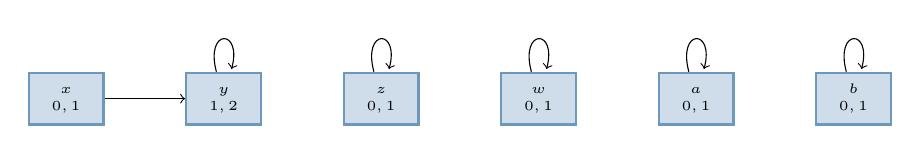
\begin{tikzpicture}[auto]

%
% Styles
%
\tikzstyle{vertex} = [rectangle,draw=oproverblue!60,fill=oproverblue!20,thick]

\node[vertex] (x) at ( 0, 0)  {$\nod{x}{0}{1}$};
\node[vertex] (y) at ( 2, 0)  {$\nod{y}{1}{2}$};
\node[vertex] (z) at ( 4, 0)  {$\nod{z}{0}{1}$};
\node[vertex] (w) at ( 6, 0)  {$\nod{w}{0}{1}$};
\node[vertex] (a) at ( 8, 0)  {$\nod{a}{0}{1}$};
\node[vertex] (b) at (10, 0)  {$\nod{b}{0}{1}$};

\draw[->] (x) -- (y);
\path (y) edge [loop above] (y);
\path (z) edge [loop above] (z);
\path (w) edge [loop above] (w);
\path (a) edge [loop above] (a);
\path (b) edge [loop above] (b);

\end{tikzpicture}

  \vfill\pause
  Processing $w=a$. State after Union( Find( $w$ ), Find( $a$ ) ) 
  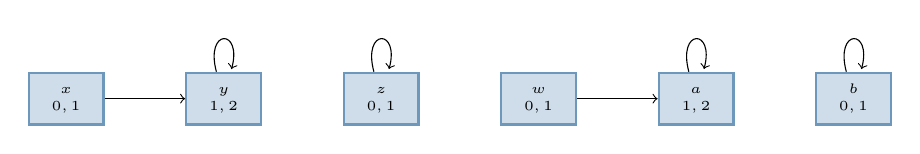
\begin{tikzpicture}[auto]

%
% Styles
%
\tikzstyle{vertex} = [rectangle,draw=oproverblue!60,fill=oproverblue!20,thick]

\node[vertex] (x) at ( 0, 0)  {$\nod{x}{0}{1}$};
\node[vertex] (y) at ( 2, 0)  {$\nod{y}{1}{2}$};
\node[vertex] (z) at ( 4, 0)  {$\nod{z}{0}{1}$};
\node[vertex] (w) at ( 6, 0)  {$\nod{w}{0}{1}$};
\node[vertex] (a) at ( 8, 0)  {$\nod{a}{1}{2}$};
\node[vertex] (b) at (10, 0)  {$\nod{b}{0}{1}$};

\draw[->] (x) -- (y);
\path (y) edge [loop above] (y);
\path (z) edge [loop above] (z);
\draw[->] (w) -- (a);
\path (a) edge [loop above] (a);
\path (b) edge [loop above] (b);

\end{tikzpicture}

  \vfill\pause
  Processing $w=b$. State after Union( Find( $w$ ), Find( $b$ ) ) 
  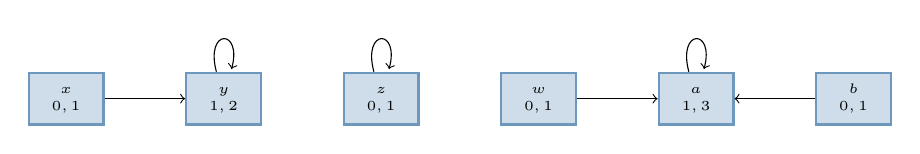
\begin{tikzpicture}[auto]

%
% Styles
%
\tikzstyle{vertex} = [rectangle,draw=oproverblue!60,fill=oproverblue!20,thick]

\node[vertex] (x) at ( 0, 0)  {$\nod{x}{0}{1}$};
\node[vertex] (y) at ( 2, 0)  {$\nod{y}{1}{2}$};
\node[vertex] (z) at ( 4, 0)  {$\nod{z}{0}{1}$};
\node[vertex] (w) at ( 6, 0)  {$\nod{w}{0}{1}$};
\node[vertex] (a) at ( 8, 0)  {$\nod{a}{1}{3}$};
\node[vertex] (b) at (10, 0)  {$\nod{b}{0}{1}$};

\draw[->] (x) -- (y);
\path (y) edge [loop above] (y);
\path (z) edge [loop above] (z);
\draw[->] (w) -- (a);
\path (a) edge [loop above] (a);
\draw[->] (b) -- (a);

\end{tikzpicture}

  \end{center}

\end{frame}

\begin{frame}
  \frametitle{Complexity}

  \scriptsize

  If we have $n$ input variables\vfill
  Union complexity: \pause $O(1)$ \\ \pause
  Find complexity: $O(\log n)$ \pause
  \vfill
  The complexity of Find is linear in the rank (height) of the trees. 
  However because Union does not increase rank unless necessary, 
  trees are always {\bf balanced}. The following invariant holds
  \begin{exampleblock}{Invariant}
    For each representant $x$, $2^{x.rank} \leq x.size$ 
  \end{exampleblock} 
  Worst case $\quad\quad x.size = n\quad\quad$ and so $\quad\quad x.rank = \log_2 n\quad\quad$ 
  \vfill\pause
  If $m$ equalities $n$ variables, worst case of $O(m\log n)$
  \vfill
  There is an improvement for Find, called {\bf path compression},
  that decrease the bound to $O(m\alpha(m,n))$, where $\alpha$ is
  the inverse of Ackermann's function ($\alpha(m,n) \leq 4$ in practice)

\end{frame}

\begin{frame}[fragile]
  \frametitle{Quick-Find approach}

  \scriptsize

  \begin{verbatim}
    struct Node { 
      int    size;     // Keep track of a class size
      Node * next;     // Next element in eq. class (circular list)
      Node * root;     // Points to class' representant
    };
  \end{verbatim} 
  initialized as size = 0, next = $x$, root = $x$
  \vfill
  \begin{columns}

  \begin{column}{.45\textwidth}
    \pause
    \begin{tabbing}
      asd \= ad \= sd \= asd \kill
      1 \> {\bf procedure} Union( $x$, $y$ ) \\
      2 \> assert( $x$ == $x$.root \&\& $y$ == $y$.root ) \\
      3 \> if ( $x$ == $y$ ) return \\
      4 \> if ( $x$.size $>$ $y$.size ) \\
      5 \> \> SWAP( $x$, $y$ ) \\
      6 \> $s = x$.next \\
      7 \> while ( $s \not= x$ ) \\
      8 \> \> $s$.root $=$ $y$ \\
      9 \> \> $s = s$.next \\
     10 \> SPLICE( $x$, $y$ ) \\
     11 \> $y$.size = $y$.size $+$ $x$.size \\
    \end{tabbing}
  \end{column}
  
  \begin{column}{.35\textwidth}
    \begin{tabbing}
      asd \= ad \= sd \= asd \kill
      1 \> {\bf procedure} Find( $x$ ) \\
      2 \> return $x.root$ \\
      \\
      \\
      1 \> {\bf procedure} Union-Find( $\varphi^+$ ) \\
      2 \> foreach ( $x=y \in \varphi^+$ ) \\  
      3 \> \> $x =$ Find( $x$ ) \\
      4 \> \> $y =$ Find( $y$ ) \\
      5 \> \> Union( $x$, $y$ )
    \end{tabbing}
  \end{column}

  \end{columns}
  \vfill\pause
  Union $O(n)$, Find $O(1)$, Union-Find $O(n\log n)$

\end{frame}

\subsection{Congruence-Closure}
\subsection{Solving}

\begin{frame}
  \frametitle{The Tableau}

  \scriptsize

  The equations $A\vec{x} = \vec{0}$ are kept in a {\bf tableau}, the most 
  important structure of the Simplex
  \vfill
  The variables are {\bf partitioned} into the set of {\bf non-basic} \nonbas
  and {\bf basic} \bas  variables 
  \vfill
  E.g., \bas = $\{ x_1, x_3, x_4 \}$, \nonbas = $\{ x_2, x_5, x_6 \}$
  $$
  \begin{array}{rcl}
    x_1 & = & 4 x_2 + x_5 \\
    x_3 & = & 5 x_2 + 3 x_6 \\
    x_4 & = & x_5 - x_6
  \end{array}
  $$
  \vfill
  non-basic variables can be considered as {\bf independent}, while basic variables
  assume values forced by the non-basic ones. E.g., in the row
  $$
    x_1 = 4 x_2 + x_5 
  $$
  suppose that $x_2 = 2, x_5 = 1$, then we set $x_1 = 9$

\end{frame}

\begin{frame}
  \frametitle{Solving}

  \scriptsize

  The \tsolver stores 
  \begin{itemize}
    \item the Tableau (does not grow/shrink)
    \item the active bounds on variables (initially none)
    \item the current model $\mu$ (initially all $0$, but could be chosen differently)
  \end{itemize}

  \vfill

  \begin{columns}

  \begin{column}{.4\textwidth}
  \begin{center}
  Tableau
  \end{center}
  $$
  \begin{array}{rcl}
    x_1 & = & a_{11} x_{m+1} \ldots + a_{1n} x_n  \\ 
    x_2 & = & a_{21} x_{m+1} \ldots + a_{2n} x_n  \\ 
    & \ldots \\                             
    x_i & = & a_{i1} x_{m+1} \ldots + a_{in} x_n  \\ 
    & \ldots \\                             
    x_m & = & a_{m1} x_{m+1} \ldots + a_{mn} x_n \\
    \\
    \\
  \end{array}
  $$
  \end{column}

  \begin{column}{.3\textwidth}
  \begin{center}
  $lb$~~~~~~~Bounds~~~~~~~$ub$
  \end{center}
  $$
  \begin{array}{rcccl}
    - \infty & \leq & x_1 & \leq & \infty \\
    - \infty & \leq & x_2 & \leq & \infty \\
    & & \ldots & & \\
    - \infty & \leq & x_i & \leq & \infty \\
    & & \ldots & & \\
    - \infty & \leq & x_m & \leq & \infty \\
    & & \ldots & & \\
    - \infty & \leq & x_n & \leq & \infty \\
  \end{array}
  $$
  \end{column}

  \begin{column}{.3\textwidth}
  \begin{center}
  $\mu$
  \end{center}
  $$
  \begin{array}{rcl}
  x_1 & \mapsto & 0 \\
  x_2 & \mapsto & 0 \\
  & \ldots \\
  x_i & \mapsto & 0 \\
  & \ldots \\
  x_m & \mapsto & 0 \\
  & \ldots \\
  x_n & \mapsto & 0 
  \end{array}
  $$
  \end{column}

  \end{columns}

  \vfill

  The \tsolver is in a consistent state if the model $(i)$ respects the tableau 
  and $(ii)$ satisfies the bounds (for all $x$, $lb(x) \leq \mu(x) \leq ub(x)$)

\end{frame}

\begin{frame}
  \frametitle{Asserting a bound on a non-basic variable}

  \scriptsize

  Asserting a bound $x \leq c$ (resp. $x \geq c$), $x \in \nonbas$ may result in \pause
  \begin{itemize}
    \item unsatisfiability, if $c < lb(x)$ (resp. $c > ub(x)$) \pause
    \item nothing, if $c > ub(x)$ (resp. $c < lb(x)$) \pause
    \item bound tightening, model not affected if $\mu(x) \leq c$ (resp. $\mu(x) \geq c$) \pause
    \item bound tightening, model affected if $\mu(x) > c$ (resp. $\mu(x) < c$) \pause
  \end{itemize}
  \vfill
  The last case is ``problematic'' because we need to 
  \begin{enumerate}[$(i)$]
    \item adjust $\mu(x)$: $\mu(x)$ is set to $c$ 
    \item adjust the values of basic variables
  \end{enumerate}
  We assume we have a function $Update(x,c)$ that implements $(i)-(ii)$
  \vfill \pause
  \begin{columns}

  \begin{column}{.4\textwidth}
  \begin{center}
  Tableau
  \end{center}
  $$
  \begin{array}{rcl}
    x_1 & = & - x_3 + x_4  \\ 
    x_2 & = &   x_3 + x_4  \\ 
    \\
    \\
  \end{array}
  $$
  \end{column}

  \begin{column}{.3\textwidth}
  \begin{center}
  $lb$~~~~~~~Bounds~~~~~~~$ub$
  \end{center}
  $$
  \begin{array}{rcccl}
    - \infty & \leq & x_1 & \leq & \infty \\
    - \infty & \leq & x_2 & \leq & \infty \\
    \only<1-9|handout:0>{-\infty}\only<10->{-8} & \leq & x_3 & \leq & \only<1-7|handout:0>{\infty}\only<8->{-4} \\
    - \infty & \leq & x_4 & \leq & \infty 
  \end{array}
  $$
  \end{column}

  \begin{column}{.3\textwidth}
  \begin{center}
  $\mu$
  \end{center}
  $$
  \begin{array}{rcl}
  x_1 & \mapsto & \only<1-8|handout:0>{0}\only<9->{4} \\
  x_2 & \mapsto & \only<1-8|handout:0>{0}\only<9->{-4} \\
  x_3 & \mapsto & \only<1-8|handout:0>{\coloneat{0}{8}}\only<9->{-4} \\
  x_4 & \mapsto & 0 
  \end{array}
  $$
  \end{column}

  \end{columns}
  \vfill
  \tsolver stack: \\
  \onslide<8->{$x_3 \leq -4$\ \ \ \ (tighten $ub(x_3)$, affects other values)\\}
  \onslide<10->{$x_3 \geq -8$\ \ \ \ (tighten $lb(x_3)$, does not affect other values)\\}
  \onslide<11->{$x_3 \leq 0$\ \ \ \ \ \  (does not tighten $ub(x_3)$)\\}

\end{frame}

\begin{frame}
  \frametitle{Asserting a bound on a basic variable}

  \scriptsize

  Asserting a bound $x \leq c$ (resp. $x \geq c$), $x \in \bas$ may result in
  the same $4$ cases as before
  \begin{itemize}
    \item unsatisfiability, if $c < lb(x)$ (resp. $c > ub(x)$) 
    \item nothing, if $c > ub(x)$ (resp. $c < lb(x)$) 
    \item bound tightening, model not affected if $\mu(x) \leq c$ (resp. $\mu(x) \geq c$)
    \item bound tightening, model affected if $\mu(x) > c$ (resp. $\mu(x) < c$) 
  \end{itemize}
  \vfill
  however, since a basic variable is {\bf dependent} from non-basic variables in the
  tableau, we cannot use function $Update$ directly. Before we need to 
  turn $x$ into a non-basic variables.
  \pause 
  \vfill
  So if $\mu(x) > c$ or $\mu(x) < c$ we have to
  \begin{enumerate}[$(i)$]
    \item {\bf turn $x$ into non-basic} (another non-basic variable will become basic instead)
    \item adjust $\mu(x)$: $\mu(x)$ is set to $c$ 
    \item adjust the values of basic variables
  \end{enumerate}
  \vfill
  Step $(i)$ is performed by a function $Pivot(x,y)$ (see next slide). Therefore asserting
  a bound on a basic variable $x$ consists in executing $Pivot(x,y)$ and then $Update(x,c)$
\end{frame}

\begin{frame}
  \frametitle{Pivoting}

  \scriptsize

  $Pivot(x,y)$ is the operation of swapping a basic variable $x$ with a non-basic variable $y$ 
  (how to choose $y$ ? See next slide)
  \vfill
  It consists of the following steps:
  \begin{enumerate}
    \item Take the row $x = a y + R$ in the tableau ($R = \mbox{rest of the polynome}$)
    \item Rewrite it as $y = \frac{x - R}{a}$
    \item Substitute $y$ with $\frac{x - R}{a}$ in all the other rows of the tableau (and simplify)
  \end{enumerate}
  \vfill\pause
  Example for $Pivot(x_1,x_3)$
  \vfill
  \ra{1.5}
  \begin{columns}

    \begin{column}{.33\textwidth}
      \begin{center}
      Step 1 
      \end{center}
      $$
      \begin{array}{rcl}
	\colone{x_1} & \colone{=} & \colone{3 x_2 + 4 x_3 - 5 x_4} \\
	x_5 & = & - x_2 - x_3 \\
	x_6 & = & 10 x_2 + 5 x_4	
      \end{array}
      $$
    \end{column}

    \begin{column}{.33\textwidth}
      \begin{center}
      Step 2 
      \end{center}
      $$
      \begin{array}{rcl}
	\colone{x_3} & \colone{=} & \colone{-\frac{3}{4} x_2 + \frac{1}{4} x_1 + \frac{5}{4} x_4} \\
	x_5 & = & - x_2 - x_3 \\
	x_6 & = & 10 x_2 + 5 x_4	
      \end{array}
      $$
    \end{column}

    \begin{column}{.33\textwidth}
      \begin{center}
      Step 3 
      \end{center}
      $$
      \begin{array}{rcl}
	x_3 & = & -\frac{3}{4} x_2 + \frac{1}{4} x_1 + \frac{5}{4} x_4 \\
	\colone{x_5} & \colone{=} & \colone{- \frac{1}{4} x_2 -\frac{1}{4} x_1 - \frac{5}{4} x_4} \\
	x_6 & = & 10 x_2 + 5 x_4	
      \end{array}
      $$
    \end{column}

  \end{columns}
  \vfill\pause
  we moved from $\bas = \{ x_1, x_5, x_6 \}$ to $\bas = \{ x_3, x_5, x_6 \}$ 

\end{frame}

\begin{frame}
  \frametitle{Choosing Pivoting Variable}

  \scriptsize

  Consider the following situation 
  \vfill
  \begin{columns}

  \begin{column}{.4\textwidth}
  \begin{center}
  Tableau
  \end{center}
  $$
  \begin{array}{rcl}
    & \ldots \\                             
    x_1 & = & 3 x_2 - 4 x_3 + 2 x_4 - x_5 \\ 
    & \ldots \\                             
    \\
    \\
  \end{array}
  $$
  \end{column}

  \begin{column}{.3\textwidth}
  \begin{center}
  $lb$~~~~~~~Bounds~~~~~~~$ub$
  \end{center}
  $$
  \begin{array}{rcccl}
     -4 & \leq & x_1 & \leq & 10 \\
      1 & \leq & x_2 & \leq & 3 \\
     -4 & \leq & x_3 & \leq & -1 \\
      1 & \leq & x_4 & \leq & 2 \\
     -1 & \leq & x_5 & \leq & 10 \\
  \end{array}
  $$
  \end{column}

  \begin{column}{.3\textwidth}
  \begin{center}
  $\mu$
  \end{center}
  $$
  \begin{array}{rcl}
  x_1 & \mapsto & \colone{12} \\
  x_2 & \mapsto & 1 \\
  x_3 & \mapsto & -1 \\
  x_4 & \mapsto & 2 \\
  x_5 & \mapsto & -1 
  \end{array}
  $$
  \end{column}

  \end{columns}
  \vfill
  which among $\nonbas = \{ x_2, x_3, x_4 \}$ do I choose for pivoting ? Clearly, the value of $\mu(x_1)$
  is too high, I have to decrease it by playing with the values of \nonbas: \pause
  \begin{itemize}
    \item $  3 x_2$ cannot decrease, as $\mu(x_2) = lb(x_2)$ and cannot be moved down \pause
    \item $- 4 x_3$ cannot decrease, as $\mu(x_3) = ub(x_3)$ and cannot be moved up \pause
    \item $  2 x_4$ can decrease, as  $\mu(x_4) = ub(x_4)$, and can be moved down \pause
    \item $-   x_5$ can decrease, as  $\mu(x_5) = lb(x_5)$, and can be moved up
  \end{itemize}
  \vfill\pause
  both $x_4$ and $x_5$ are therefore good candidates for pivoting. To avoid loops, 
  choose variable with smallest subscript (Bland's Rule). This rule is not necessarily
  efficient, though

\end{frame}

\begin{frame}
  \frametitle{Detect Unsatisfiability}

  \scriptsize

  There might be cases in which {\bf no suitable variable for pivoting can be found}.
  This indicates unsatisfiability. \pause
  Consider the following where we have just asserted $x_1 \leq 9$
  \vfill
  \begin{columns}

  \begin{column}{.4\textwidth}
  \begin{center}
  Tableau
  \end{center}
  $$
  \begin{array}{rcl}
    & \ldots \\                             
    x_1 & = & 3 x_2 - 4 x_3 + 2 x_4 - x_5 \\ 
    & \ldots \\                             
    \\
    \\
  \end{array}
  $$
  \end{column}

  \begin{column}{.3\textwidth}
  \begin{center}
  $lb$~~~~~~~Bounds~~~~~~~$ub$
  \end{center}
  $$
  \begin{array}{rcccl}
     -4 & \leq & x_1 & \leq & 9 \\
      1 & \leq & x_2 & \leq & 3 \\
     -4 & \leq & x_3 & \leq & -1 \\
      2 & \leq & x_4 & \leq & 2 \\
     -1 & \leq & x_5 & \leq & -1 \\
  \end{array}
  $$
  \end{column}

  \begin{column}{.3\textwidth}
  \begin{center}
  $\mu$
  \end{center}
  $$
  \begin{array}{rcl}
  x_1 & \mapsto & \colone{12} \\
  x_2 & \mapsto & 1 \\
  x_3 & \mapsto & -1 \\
  x_4 & \mapsto & 2 \\
  x_5 & \mapsto & -1 
  \end{array}
  $$
  \end{column}

  \end{columns}
  \vfill
  no variable among $\nonbas = \{ x_2, x_3, x_4 \}$ can be chosen for pivoting. This is because (due to tableau)
  $$x_2 \geq 3\ \swedge\ x_3 \leq -1\ \swedge\ x_4 \geq 4\ \swedge\ x_5 \leq -1\ \ \Rightarrow\ \ x_1 \geq 12\ \ \Rightarrow\ \ \neg (x_1 \leq 9)$$
  \vfill
  Therefore
  $$\{ x_2 \geq 3,\ x_3 \leq -1,\ x_4 \geq 4,\ x_5 \leq -1,\ \neg( x_1 \leq 9 ) \}$$
  is a \tconflict (modulo the tableau)

\end{frame}

\begin{frame}
  \frametitle{Solving}

  \scriptsize

  \begin{tabbing}
  asv \= a \= a \= a \= as \= asdfasdfasdfasdfasdfasdfasdfasdf \= \kill
  1  \> while( $true$ ) \\
     \> \\
  2  \> \> pick first $x_i \in \bas$ such that $\mu(x_i) < lb(x_i)$ or $\mu(x_i) > ub(x_i)$ \\
  3  \> \> if ( there is no such $x_i$ ) return $sat$ \\
     \> \\
  4  \> \> $x_j = ChoosePivot( x_i )$ \\
  5  \> \> if ( $x_j$ == $undef$ ) return $unsat$ \\ 
  6  \> \> $Pivot(x_i,x_j)$ \\
     \> \\
  7  \> \> if ( $\mu(x_i) < lb(x_i)$ ) \\
  8  \> \> \> $Update( x_i, lb(x_i) )$ \\
     \> \\
  9  \> \> if ( $\mu(x_i) > ub(x_i)$ ) \\
  10 \> \> \> $Update( x_i, ub(x_i) )$ \\
     \> \\
  11 \> end
  \end{tabbing}

  $x_j = ChoosePivot( x_i )$: returns variable to use for pivoting with $x_i$, or $undef$ if conflict\\
  pick first $x_i$ \ldots: it's again Bland's rule

\end{frame}


\section{\tsolver for \Uf}
\subsection{\tsolver features}
\begin{frame}
  \frametitle{\tsolver features}

  \begin{itemize}

  \item Incrementality: for free, as Congruence-Closure is already incremental

  \vfill\pause

  \item Backtrackability: backtracking one equality amounts to {\bf undo} 
                          all the operations done during Congruence-Closure.
			  (This means that backtracking is as expensive as
			  solving)

  \vfill\pause

  \item Minimal \tconflicts: computing minimal conflicts in \Uf is theoretically
                             very hard (NP-complete). We'll an acceptable way to
			     compute them

  \vfill\pause

  \item Theory-Propagation: it amounts to track all unassigned equalities such
                            as $a=b$. If during some Union( $x$, $y$ ), $a$ 
			    and $b$ become equal (because for instance 
			    $a$ is in the class of $x$ and $b$ is in the class
			    of $y$), then propagate $a=b$

  \end{itemize}

\end{frame}

\subsection{Computing \tconflicts}
\begin{frame}
  \frametitle{Computing \tconflicts}

  \scriptsize

  First of all notice that \tconflicts are always of the form
  $$
    \{\ s \not= t, \mbox{``other equalities that cause } s \mbox{ and } t \mbox{ to join the same class''} \} 
  $$
  We reconstruct the conflict by storing the reason that caused two classes to collapse. When a
  $s \not=t $ causes $unsat$, we call a routine Explain($s$,$t$) that collects all the reasons
  that made $s$ equal to $t$ \\
  Example 
  $$
  \{\ \coloneat{x\!=\!y}{2}
   ,\ \coloneat{y\!=\!w}{3}
   ,\ \coloneat{f(x)\!=\!z}{5}
   ,\ \coloneat{f(w)\!=\!a}{6}
   ,\ \coloneat{a\!\not=\!z}{7-}\ \}
  $$
  \begin{overlayarea}{\textwidth}{3cm}
    \begin{center}
    \only<1|handout:0>{
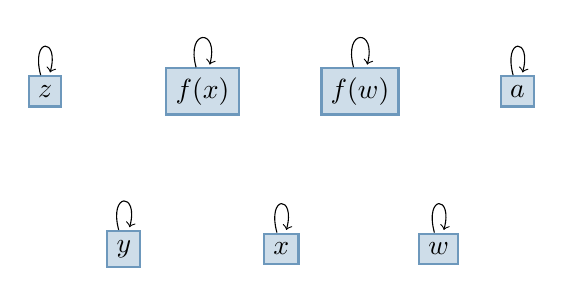
\begin{tikzpicture}[auto]

%
% Styles
%
\tikzstyle{vertex} = [rectangle,draw=oproverblue!60,fill=oproverblue!20,thick]

\node[vertex] (y) at  (  2, 0)  {$y$};
\node[vertex] (x) at  (  4, 0)  {$x$};
\node[vertex] (w) at  (  6, 0)  {$w$};
\node[vertex] (fx) at (  3, 2)  {$f(x)$};
\node[vertex] (fw) at (  5, 2)  {$f(w)$};
\node[vertex] (z) at  (  1, 2)  {$z$};
\node[vertex] (a) at  (  7, 2)  {$a$};

\path (x)  edge [loop above] (x);
\path (y)  edge [loop above] (y);
\path (z)  edge [loop above] (z);
\path (w)  edge [loop above] (w);
\path (a)  edge [loop above] (a);
\path (fx) edge [loop above] (fx);
\path (fw) edge [loop above] (fw);

\end{tikzpicture}
}
    \only<2|handout:0>{
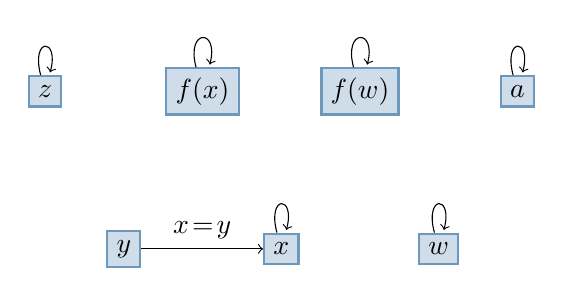
\begin{tikzpicture}[auto]

%
% Styles
%
\tikzstyle{vertex} = [rectangle,draw=oproverblue!60,fill=oproverblue!20,thick]

\node[vertex] (y) at  (  2, 0)  {$y$};
\node[vertex] (x) at  (  4, 0)  {$x$};
\node[vertex] (w) at  (  6, 0)  {$w$};
\node[vertex] (fx) at (  3, 2)  {$f(x)$};
\node[vertex] (fw) at (  5, 2)  {$f(w)$};
\node[vertex] (z) at  (  1, 2)  {$z$};
\node[vertex] (a) at  (  7, 2)  {$a$};

\draw[->] (y)  -- node {$x\!=\!y$} (x);
\path (x)  edge [loop above] (x);
\path (z)  edge [loop above] (z);
\path (w)  edge [loop above] (w);
\path (a)  edge [loop above] (a);
\path (fx) edge [loop above] (fx);
\path (fw) edge [loop above] (fw);

\end{tikzpicture}
}
    \only<3|handout:0>{
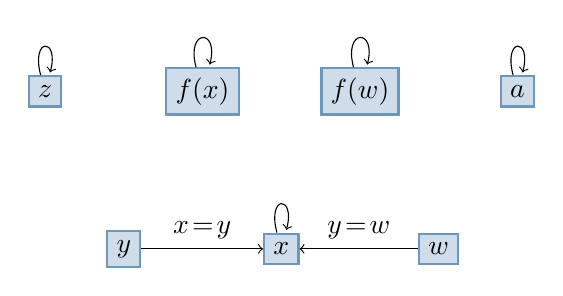
\begin{tikzpicture}[auto]

%
% Styles
%
\tikzstyle{vertex} = [rectangle,draw=oproverblue!60,fill=oproverblue!20,thick]

\node[vertex] (y) at  (  2, 0)  {$y$};
\node[vertex] (x) at  (  4, 0)  {$x$};
\node[vertex] (w) at  (  6, 0)  {$w$};
\node[vertex] (fx) at (  3, 2)  {$f(x)$};
\node[vertex] (fw) at (  5, 2)  {$f(w)$};
\node[vertex] (z) at  (  1, 2)  {$z$};
\node[vertex] (a) at  (  7, 2)  {$a$};

\draw[->] (y)  -- node {$x\!=\!y$} (x);
\draw[->] (w)  -- node[above] {$y\!=\!w$} (x);
\path (z)  edge [loop above] (z);
\path (x)  edge [loop above] (x);
\path (a)  edge [loop above] (a);
\path (fx) edge [loop above] (fx);
\path (fw) edge [loop above] (fw);

\end{tikzpicture}
}
    \only<4|handout:0>{
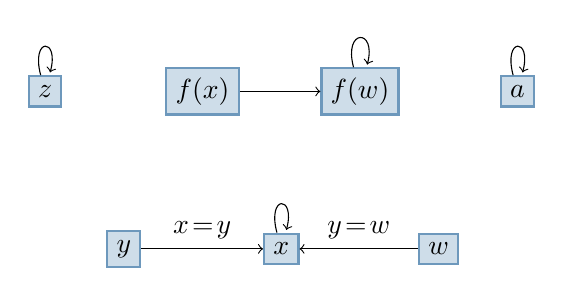
\begin{tikzpicture}[auto]

%
% Styles
%
\tikzstyle{vertex} = [rectangle,draw=oproverblue!60,fill=oproverblue!20,thick]

\node[vertex] (y) at  (  2, 0)  {$y$};
\node[vertex] (x) at  (  4, 0)  {$x$};
\node[vertex] (w) at  (  6, 0)  {$w$};
\node[vertex] (fx) at (  3, 2)  {$f(x)$};
\node[vertex] (fw) at (  5, 2)  {$f(w)$};
\node[vertex] (z) at  (  1, 2)  {$z$};
\node[vertex] (a) at  (  7, 2)  {$a$};

\draw[->] (y)  -- node {$x\!=\!y$} (x);
\draw[->] (w)  -- node[above] {$y\!=\!w$} (x);
\path (z)  edge [loop above] (z);
\path (x)  edge [loop above] (x);
\path (a)  edge [loop above] (a);
\draw[->] (fx) -- (fw);
\path (fw) edge [loop above] (fw);

\end{tikzpicture}
}
    \only<5|handout:0>{
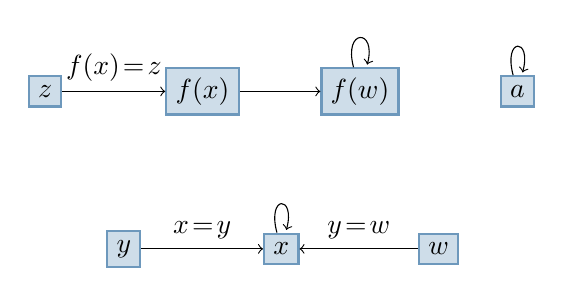
\begin{tikzpicture}[auto]

%
% Styles
%
\tikzstyle{vertex} = [rectangle,draw=oproverblue!60,fill=oproverblue!20,thick]

\node[vertex] (y) at  (  2, 0)  {$y$};
\node[vertex] (x) at  (  4, 0)  {$x$};
\node[vertex] (w) at  (  6, 0)  {$w$};
\node[vertex] (fx) at (  3, 2)  {$f(x)$};
\node[vertex] (fw) at (  5, 2)  {$f(w)$};
\node[vertex] (z) at  (  1, 2)  {$z$};
\node[vertex] (a) at  (  7, 2)  {$a$};

\draw[->] (y)  -- node {$x\!=\!y$} (x);
\draw[->] (w)  -- node[above] {$y\!=\!w$} (x);
\draw[->] (z)  -- node {$f(x)\!=\!z$} (fx);
\path (x)  edge [loop above] (x);
\path (a)  edge [loop above] (a);
\draw[->] (fx) -- (fw);
\path (fw) edge [loop above] (fw);

\end{tikzpicture}
}
    \only<6->{
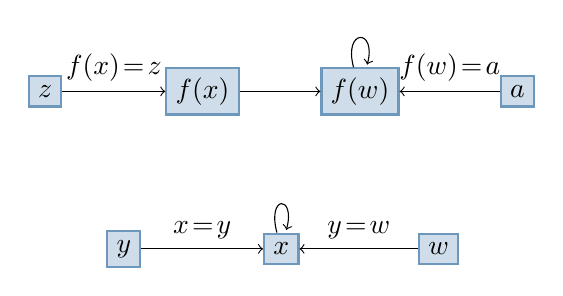
\begin{tikzpicture}[auto]

%
% Styles
%
\tikzstyle{vertex} = [rectangle,draw=oproverblue!60,fill=oproverblue!20,thick]

\node[vertex] (y) at  (  2, 0)  {$y$};
\node[vertex] (x) at  (  4, 0)  {$x$};
\node[vertex] (w) at  (  6, 0)  {$w$};
\node[vertex] (fx) at (  3, 2)  {$f(x)$};
\node[vertex] (fw) at (  5, 2)  {$f(w)$};
\node[vertex] (z) at  (  1, 2)  {$z$};
\node[vertex] (a) at  (  7, 2)  {$a$};

\draw[->] (y)  -- node {$x\!=\!y$} (x);
\draw[->] (w)  -- node[above] {$y\!=\!w$} (x);
\draw[->] (z)  -- node {$f(x)\!=\!z$} (fx);
\path (x)  edge [loop above] (x);
\path (fw)  edge [loop above] (fw);
\draw[->] (fx) -- (fw);
\draw[->] (a) -- node[above] {$f(w)\!=\!a$} (fw);

\end{tikzpicture}
}
    \end{center}
  \end{overlayarea}
  \vfill
  \onslide<7->{
  On processing $a\not=z$, we call Explain( $a$, $z$ )
  }

\end{frame}

\begin{frame}
  \frametitle{Computing \tconflicts}

  \scriptsize

  $$
  \{\ x\!=\!y
   ,\ y\!=\!w
   ,\ f(x)\!=\!z
   ,\ f(w)\!=\!a
   ,\ a\!\not=\!z\ 
  \}
  $$
  \begin{center}
  
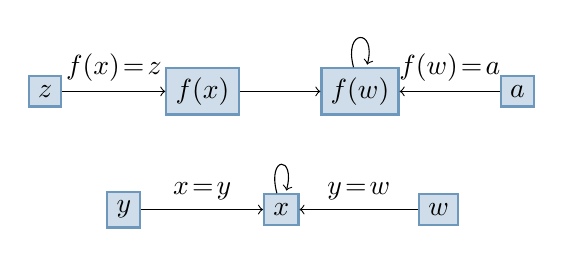
\begin{tikzpicture}[auto]

%
% Styles
%
\tikzstyle{vertex} = [rectangle,draw=oproverblue!60,fill=oproverblue!20,thick]

\node[vertex] (y) at  (  2, 0)  {$y$};
\node[vertex] (x) at  (  4, 0)  {$x$};
\node[vertex] (w) at  (  6, 0)  {$w$};
\node[vertex] (fx) at (  3, 1.5)  {$f(x)$};
\node[vertex] (fw) at (  5, 1.5)  {$f(w)$};
\node[vertex] (z) at  (  1, 1.5)  {$z$};
\node[vertex] (a) at  (  7, 1.5)  {$a$};

\draw[->] (y)  -- node {$x\!=\!y$} (x);
\draw[->] (w)  -- node[above] {$y\!=\!w$} (x);
\draw[->] (z)  -- node {$f(x)\!=\!z$} (fx);
\path (x)  edge [loop above] (x);
\path (fw)  edge [loop above] (fw);
\draw[->] (fx) -- (fw);
\draw[->] (a) -- node[above] {$f(w)\!=\!a$} (fw);

\end{tikzpicture}

  \end{center}
  \vfill
  If $a$ and $z$ are in the same class, it means that there are paths of the form
  $$a \rightarrow^* u\quad\quad z \rightarrow^* u$$ 
  (it could happen that $u \equiv a$ or $u \equiv z$)
  \vfill\pause
  Explain( $s$, $t$ ) intuitively works as follows:
  \begin{enumerate}
    \item Traverse $s \rightarrow^* u$ and collect all labels on edges
    \item Traverse $t \rightarrow^* u$ and collect all labels on edges
    \item If during collection an empty label was found
    \begin{enumerate}
      \scriptsize
      \item It must be some $f(s_1,\ldots,s_n) \rightarrow f(t_1,\ldots,t_n)$
      \item call Explain( $s_i$, $t_i$ ) for $i \in [1..n]$
    \end{enumerate}
    \item At the end of the recursions, the collected labels (without repetitions)
          are a \tconflict
  \end{enumerate}

\end{frame}

\subsection{Final remarks}
\begin{frame}
  \frametitle{Final Remarks}

  We did not say how to handle negative \tatoms, such as $\neg( x - y \leq c )$.
  However it is easy to see that  $\quad\neg( x - y \leq c )\quad$ iff $\quad y  - x \leq - c - 1\quad$
  \vfill
  Each \tatom is associated to two edges $(x,y;c), (y,x;-c-1)$. However
  at most only one of the two is activated (depending if \tatom is pushed positively or
  negatively)
  \vfill
  \pause
  Simple bounds, such as $\quad x \leq c\quad$ or $\quad - x \leq c\quad$ can also be handled. It is
  sufficient to add a ``fake'' (and fresh) variable $Z$ (stands for ``zero''),
  and use $\quad x - Z \leq c\quad$ and $\quad Z - x \leq c\quad$ instead of the above

\end{frame}

\begin{frame}
  \frametitle{Floyd-Warshall}

  Another algorithm that can be used instead of BF is the
  Floyd-Warshall
  \vfill
  FW has a complexity of $\theta(n^3)$, while BF of $O(nm)$
  (variations of BF have complexity $O(m + n \log n)$)
  \vfill
  FW however is useful as it is trivial to compute all
  theory propagations. In BF, theory propagations are tricky
  to discover
  \vfill
  FW is independent of $m$, the numeber of edges. FW is good
  for {\bf dense} problems, while is likely to be bad for
  {\bf sparse} ones

\end{frame}

\begin{frame}
  \frametitle{Exercizes}

  \begin{enumerate}

    \item Prove that adding $\{ (I,x_1;0), \ldots, (I,x_n;0) \}$ to a graph
          free of negative cycles, does not introduce any negative cycle

    \vfill

    \item Let $G(V,E)$ be a graph, let $x,y \in V$, and suppose that
          a path $y \rightarrow \ldots \rightarrow x$ exists in $G$.
	  Are the following true or false ? (if false, show counterexamples)

    \vfill

    \begin{enumerate}[$(a)$]

      \item Adding an edge $(x,y;100)$ to $G$ never causes the creation of a negative cycle 

      \item Adding an edge $(x,y;-100)$ to $G$ always causes the creation of a negative cycle 

    \end{enumerate}

    \vfill

    \item Let $\babst{\mu}$ be a set of constraints of the form $x - y \leq c$. Let
          $\mu$ be a model. Let $\zeta(x) = \{ \mu(x) + \epsilon \}$, 
	  for some $\epsilon \in \mathbb{Z}$. Show that $\zeta$  is also a model

    \vfill

    \item Show that conflicts returned discovered with checkNegativeCycle
          are always minimal

    \vfill

    \item Prove Observation 2 using Farka's Lemma

  \end{enumerate}

\end{frame}


\end{document}
